

\documentclass{article}
\usepackage[utf8]{inputenc}
% Better font encoding for French and scalable fonts
\usepackage[T1]{fontenc}
\usepackage{lmodern}
\usepackage{amsmath, amssymb, amsfonts, amsthm, stmaryrd}
\usepackage{tikz}
\usetikzlibrary{matrix,arrows}
\usepackage{tikz-cd}
\usepackage{geometry}
\usepackage[french]{babel}
\usepackage{amsopn}

\title{Étude de manoeuvres orbitales de satellites - draft}
\author{Etienne Chevrolat}
\date{}


\begin{document}

\maketitle

\begin{abstract}
    Dans cette étude, on cherche à caractériser les différents Patterns of Life (PoL) de satellites en orbites géosynchrone (GEO) et basse altitude (LEO).
    Pour cela, on se base sur de l'analyse de données TLE issues de SpaceTrack ainsi que sur le travail de chercheurs au MIT ArcLab, premiers concepteurs d'un dataset public GEO labellisé, SPLID.
    Cependant, il est bon de noter que le dataset SPLID contient des données majoritairement simulées. Nous allons donc ici nous inspirer de leur travail pour tenter de caractériser des PoL de données réelles issues de satellites en orbites GEO et LEO.
\end{abstract}

\section{Le type de données }

\subsection{Les paramètres orbitaux}

Les orbites des satellites sont elliptiques, caractérisées par leurs éléments keplériens :

\vspace{0.3cm}
\noindent\fbox{%
\begin{minipage}{0.98\textwidth}

\textbf{Paramètres orbitaux}
\begin{itemize}
    \item a : semi-grand axe de l'ellipse
    \item e : eccentricité de l'ellipse
    \item i : inclinaison de l'ellipse
    \item $\omega$ : argument du périgée
    \item $\Omega$ : Right Ascension of Ascending Node
    \item M : anomalie moyenne, renseigne sur la position du satellite sur son orbite à un instant t 
\end{itemize}
\end{minipage}

}
\vspace{0.5cm}

On peut ensuite lier des variations de vitesse dans le référentiel inertiel terrestre aux variations des paramètres orbitaux de l'ellipse, et vice-versa. 

\vspace{0.3cm}

\noindent\fbox{
\begin{minipage}{0.98\textwidth}
\textbf{Variations de vitesse et variations de paramètres orbitaux}\newline
On considère une variation $\Delta v = (\Delta v _r , \Delta v _u ,\Delta v _h )$ de la vitesse décomposée dans le référentiel terrestre en vitesses radiale, tangentielle et normale.
Les équations de Gauss nous donnent dans la limite quasi-circulaire:  
\begin{itemize}
    \item $\Delta a = \dfrac{2}{n} \Delta v _u$
    \item $\Delta e = \dfrac{1}{na}(\sin f \Delta v _r  + 2 \cos f \Delta v_u )$
    \item $\Delta i = \dfrac{1}{na}(\cos (\omega + f)  \Delta v _h  )$
    \item $\Delta \Omega  = \dfrac{1}{na}(\dfrac{\sin (\omega + f )}{\sin i }\Delta v _h  )$
    \item $\Delta \omega =  \dfrac{1}{na e }( - \cos f \Delta v _r   + 2 \sin f \Delta v_u ) - \Delta \Omega \cos i $
\end{itemize}
\end{minipage}

}
\vspace{0.3cm}

On en déduit les interprétations suivantes : 
Des variations de a et e traduisent des manoeuvres \textit{in plane}  (variation de vitesse radiale)
Des variations de i et $\Omega$ traduisent des  manoeuvres \textit{out plane} (variation de vitesse normale)

\subsection{Two Line Elements}

Les paramètres orbitaux décrits ci-dessus ne sont pas mesurés directement : ils sont diffusés par les organismes de surveillance de l'espace sous la forme de \textit{Two Line Elements} (TLE).
Un TLE est un format standardisé qui encode, sur deux lignes de 69 caractères, l'ensemble des éléments nécessaires pour reconstituer l'orbite d'un objet à un instant de référence appelé \textit{epoch}.

\vspace{0.3cm}
\noindent\fbox{%
\begin{minipage}{0.98\textwidth}

\textbf{Contenu d'un TLE}
\begin{itemize}
    \item \textbf{Identification} : numéro de catalogue NORAD, classification, désignateur international (année de lancement, numéro de lancement) et numéro du jeu d'éléments.
    \item \textbf{Epoch} : date de référence à laquelle les éléments sont valides, exprimée en année et fraction de jour.
    \item \textbf{Éléments orbitaux} : inclinaison $i$, ascension droite du noeud ascendant $\Omega$, eccentricité $e$, argument du périgée $\omega$, anomalie moyenne $M$ et moyen mouvement $n$ (en révolutions par jour).
    \item \textbf{Termes de perturbation} : dérivées première et seconde du moyen mouvement ($\dot n$, $\ddot n$) et coefficient de traînée atmosphérique $B^*$.
\end{itemize}
\end{minipage}

}
\vspace{0.5cm}

Il est important de noter que les éléments contenus dans un TLE ne sont pas des éléments osculateurs (l'orbite képlérienne instantanée), mais des \textit{éléments moyens} : les perturbations périodiques à courte période en ont été retirées.
Ils ne sont donc exploitables qu'avec le modèle de propagation qui a servi à les générer.

Ce modèle est le \textbf{SGP4} (\textit{Simplified General Perturbations 4}), un propagateur analytique qui prend en entrée un TLE et fournit la position et la vitesse du satellite dans le référentiel inertiel terrestre à n'importe quel instant.
Contrairement à une simple propagation képlérienne, SGP4 tient compte des principales perturbations subies par l'orbite : l'aplatissement terrestre (harmoniques zonaux $J_2$, $J_3$, $J_4$), la traînée atmosphérique via le terme $B^*$ ainsi que les effets à longue période.


\section{Caractérisation de PoL}
\par 
On se base sur l'API SpaceTrack pour récupérer les données souhaitées sous format TLE. Cet outil a été créé pour avoir un contrôle maximal sur les données récupérées.
Lors de la requête, on peut choisir le pays d'origine des satellites ainsi que la constellation à laquelle ils appartiennent, si elle est documentée publiquement (par exemple Starlink ou OneWeb).
On peut également choisir les dates de début et de fin d'acquisition si l'on veut constituer un historique de données orbitales.
Enfin, on peut choisir la range du demi-grand axe des orbites récupérées, ce qui permet d'obtenir uniquement des données de satellites en LEO, MEO ou géostationnaires.

\subsection{Données GEO}

\par       
Un type de donnée particulièrement important pour nous est celui des satellites géostationnaires.
Leur orbite est théoriquement fixée à 35 786km au dessus de la Terre soit un rayon de l'orbite de 42 164km. 
Une fois placé sur cette orbite, le satellite est quasi-immobile dans le référentiel terrestre, ce qui lui permet de suivre une position fixe de latitude et longitude. 
La non-sphéricité de la Terre et le fait que les orbites ne soient pas purement circulaires (eccentricité très faible mais non nulle) imposent cependant une dérive de certains paramètres orbitaux.

Pour maintenir les satellites GEO sur leur position souhaitée, les opérateurs peuvent effectuer des manoeuvres dites de station-keeping :

\begin{itemize}
    \item Est-Ouest (manoeuvres in plane)
    \item Nord-Sud (manoeuvres out plane)
\end{itemize}

\par 
Des chercheurs du MIT ArcLab ont défini le premier jeu de données de manoeuvres labellisé de satellites GEO (SPLID) conséquent,
dans le but de fournir un dataset utilisable pour entrainer des modèles à reconnaitre les différentes manoeuvres.
Ils ont ainsi défini un certain nombre de PoL résumés dans la Table.1:

\begin{center}
    \includegraphics[scale=0.3]{Capture d’écran 2026-07-01 à 14.41.14.png}
\end{center}

On trace ci-dessous les paramètres orbitaux et différents noeuds correspondant aux PoL du satellite Horizons 2, NORAD 32388.
Les lignes verticales correspondent aux différents noeuds de PoL tandis que les marqueurs circulaires indiquent les PoL directionnels dans leurs domaines respectifs.
\begin{center}
    \includegraphics[scale=0.7]{Capture d’écran 2026-07-01 à 14.41.03.png}
\end{center}

Voici un résumé des noeuds de PoL d'un satellite du dataset.

\begin{center}
    \includegraphics[scale=0.4]{Capture d’écran 2026-07-01 à 14.41.33.png}
\end{center}

\subsubsection{Manoeuvres de station-keeping des satellites GEO}

On essaye maintenant de se focaliser sur des manoeuvres de type station-keeping issues de données réelles. On a d'ores et déjà constitué un dataset exploitable de l'historique de TLE de ~200 satellites GEO issus de tous les pays.
On examine deux satellites en guise d'exemple :
\begin{itemize}
    \item 43226 : Satellite US. "GOES-17 is a geostationary weather satellite designed to improve the forecasts of weather, ocean, and environment by providing faster and more detailed data, real-time images of lightning, and advanced monitoring of solar activities and space weather"
    \item  66142 : Satellite Chinois (aucune info)
\end{itemize}

On trace alors leur demi-grand axe $a$ et le résultat de notre V1 de 3 outils de détection de manoeuvres.

\begin{center}
    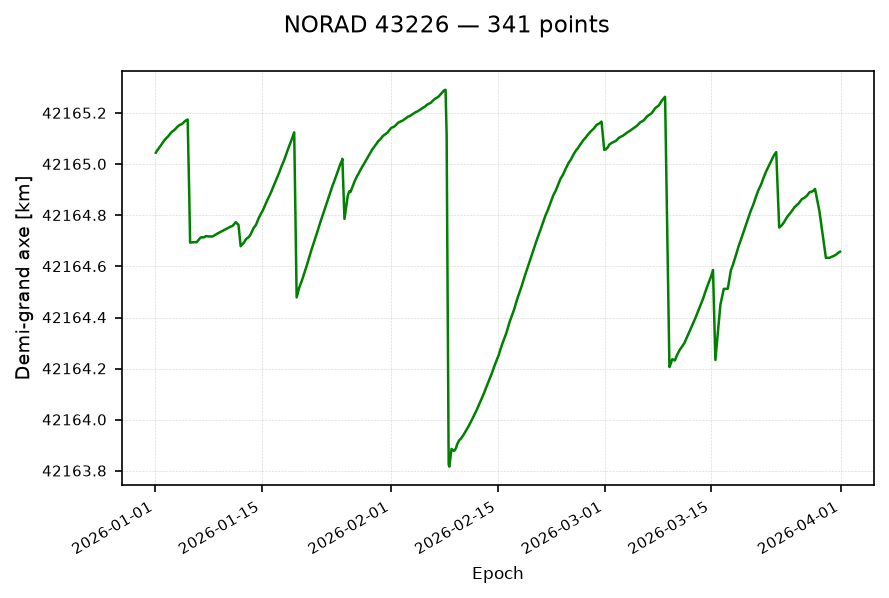
\includegraphics[scale=0.6]{norad_43226_sma.png}
    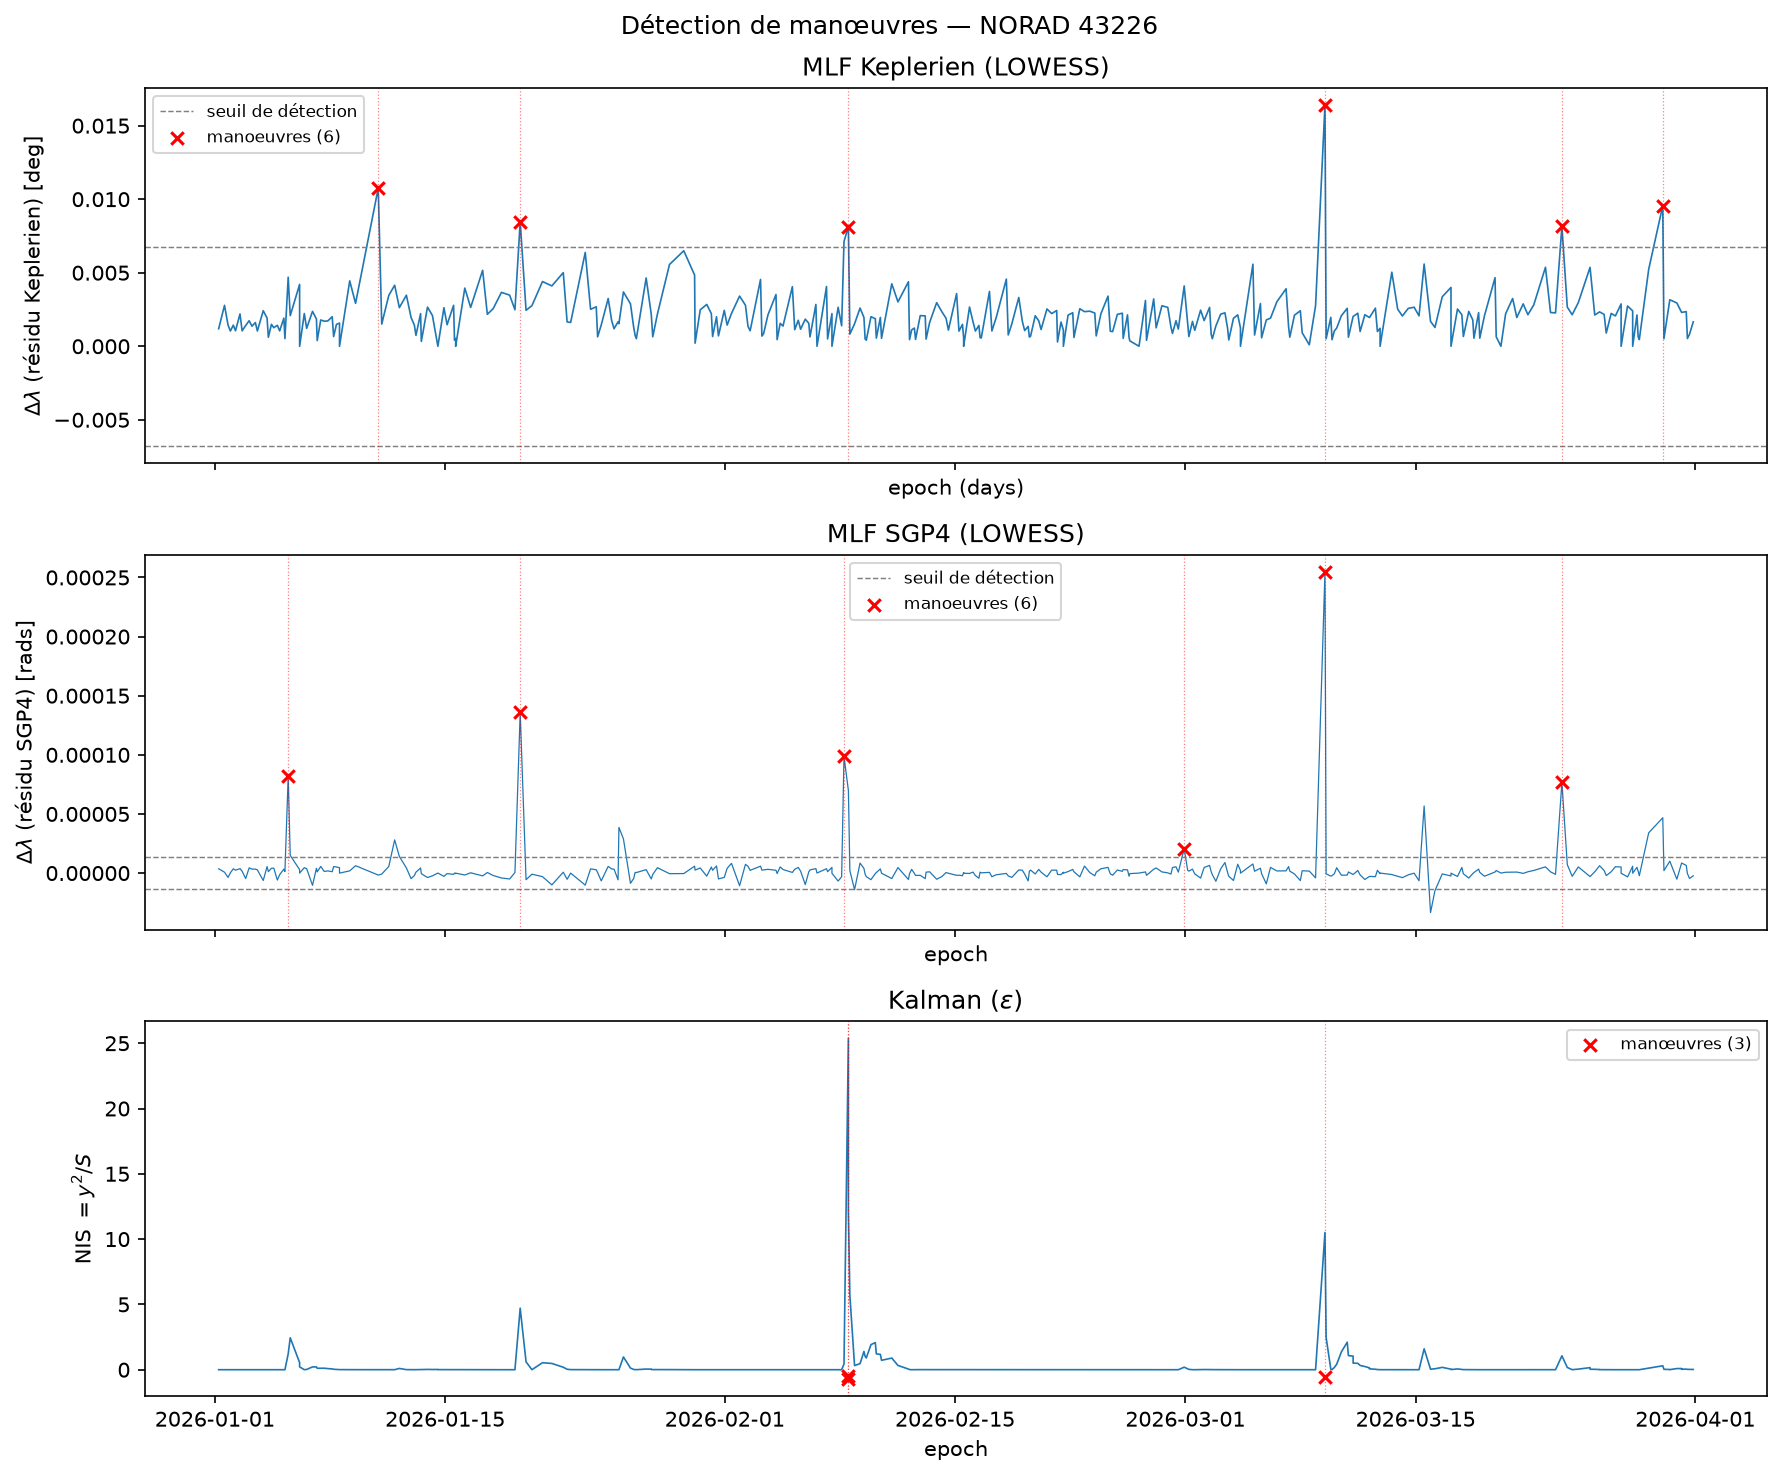
\includegraphics[scale=0.4]{norad_43226_manoeuvres.png}
\end{center}

\begin{center}
    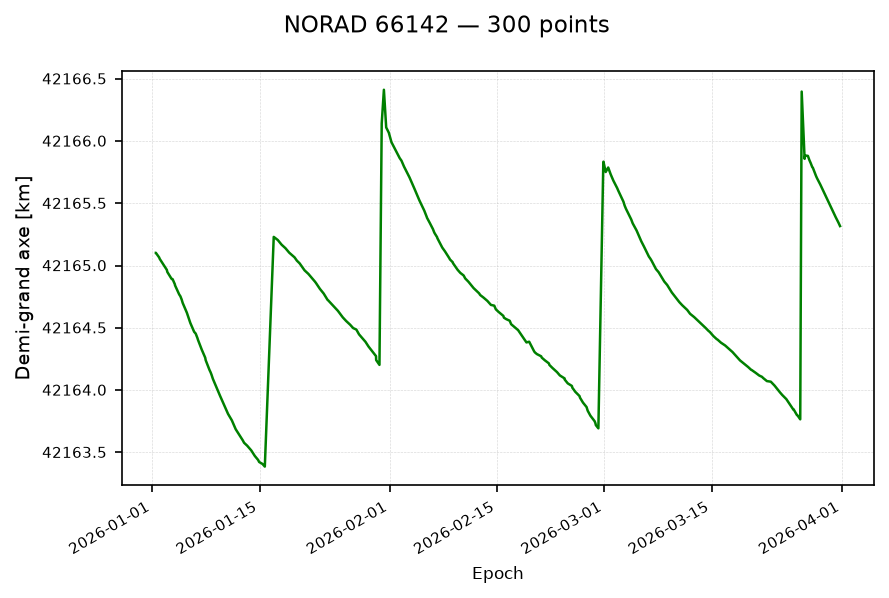
\includegraphics[scale=0.6]{norad_66142_sma.png}
    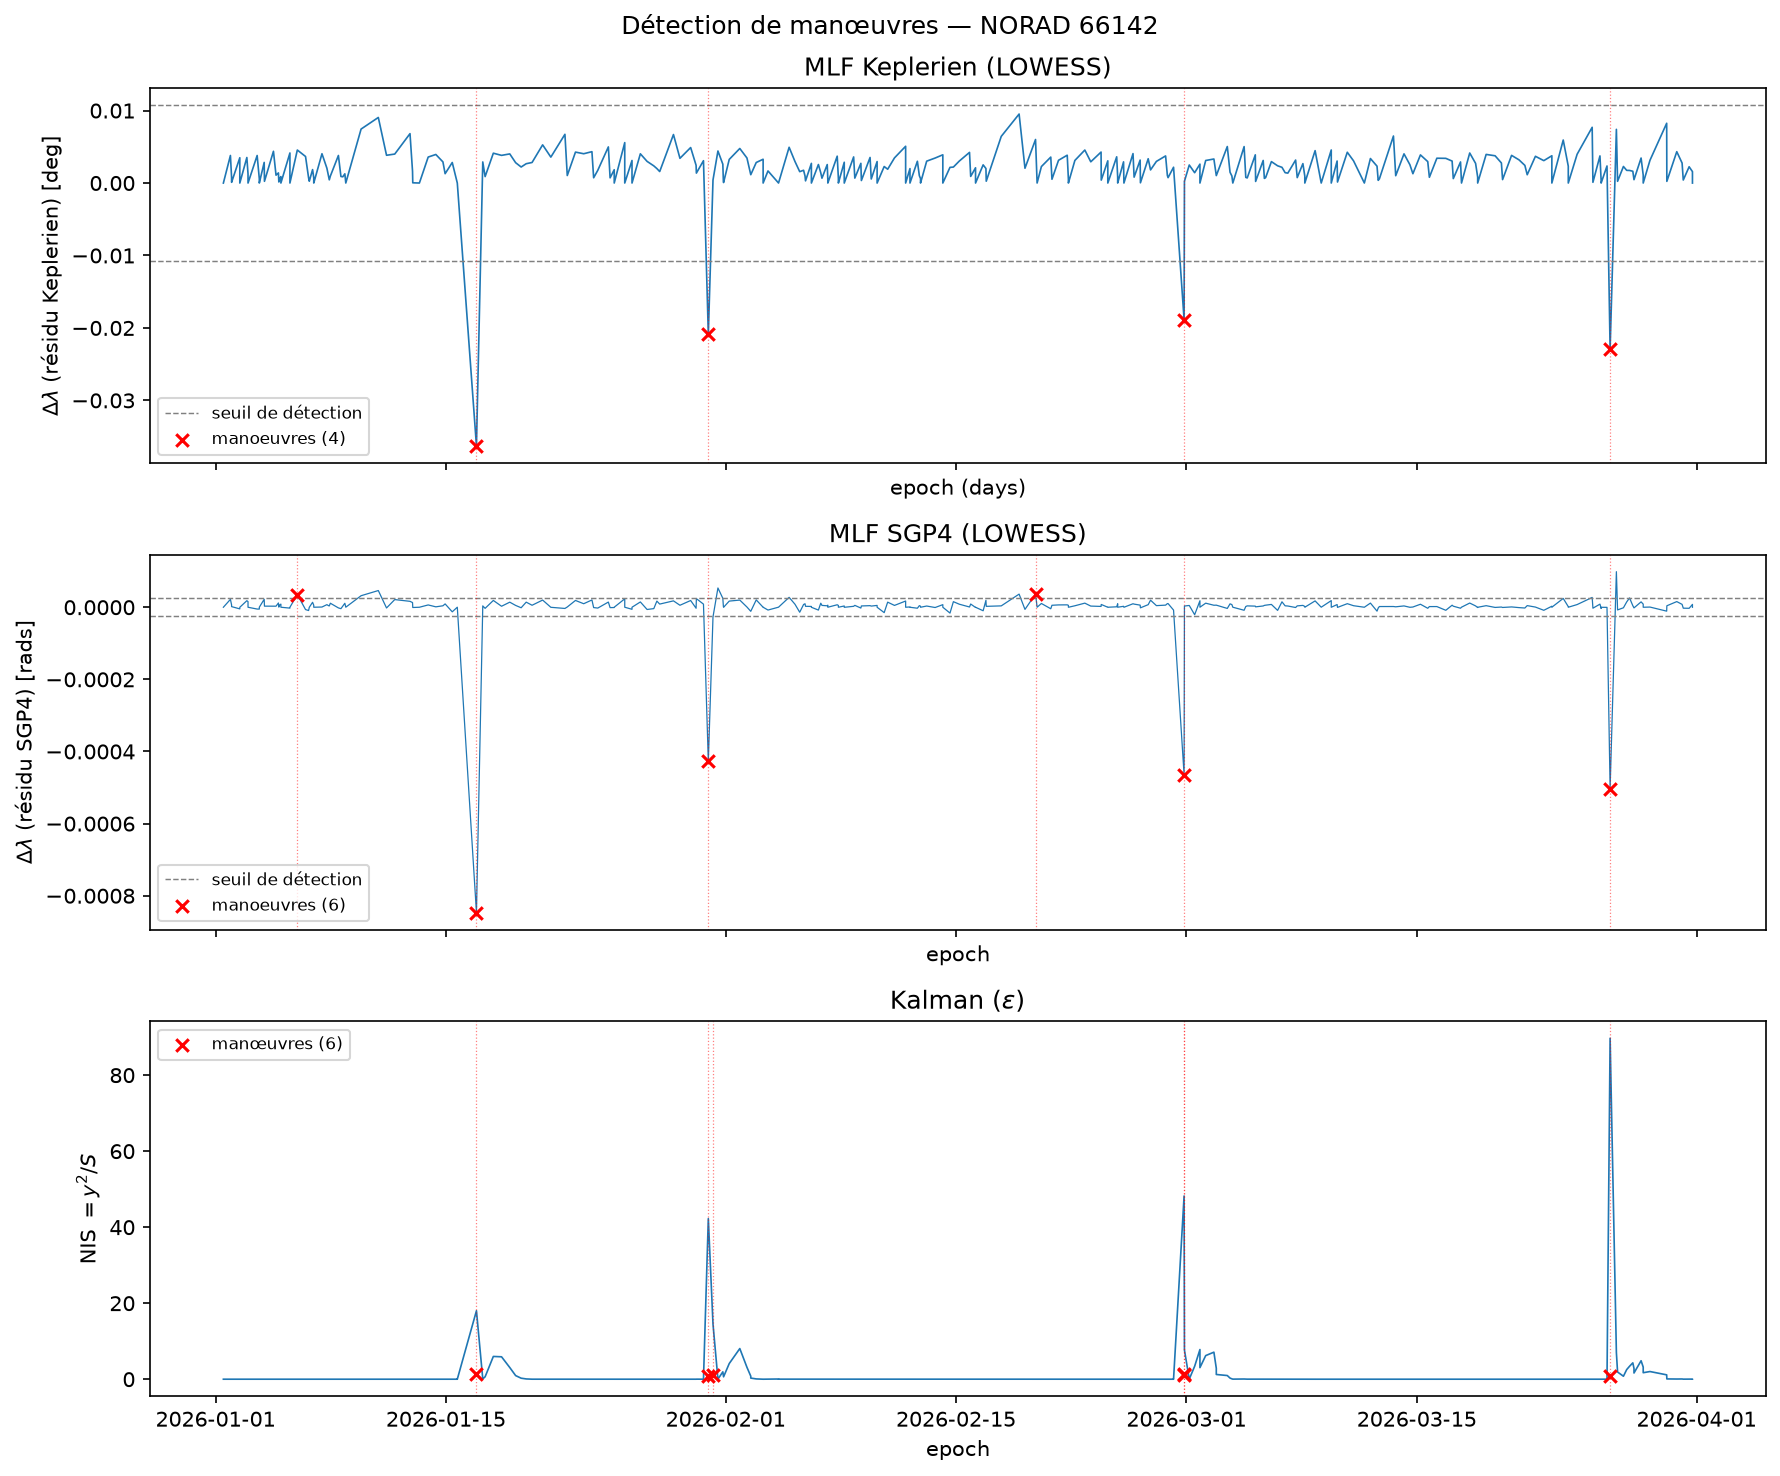
\includegraphics[scale=0.4]{norad_66142_manoeuvres.png}
\end{center}

\textbf{Remarques :}
Pour l'instant, on ne différencie pas le type de manoeuvres détectées grâce à ces différentes méthodes.
Cependant, la méthode par filtrage de Kalman est basée sur le demi-grand axe : on est donc en train de mesurer des manoeuvres in-plane.
Les méthodes Mean Longitude Filter sont basées sur la longitude moyenne $\lambda = \Omega + \omega + M$ et détectent aussi des manoeuvres in plane. 

\section{A suivre :} 
\begin{itemize}
    \item en GEO, les algos de détection de manoeuvres doivent préciser clairement le type de manoeuvres opérées (NS, EW, Station-Keeping ou non). 
    \item poursuivre l'étude de PoL en LEO, plus complexes a priori, contiennent pas seulement des manoeuvres de station-keeping
    \item effectuer des mesures quantitatives de manoeuvres (intensité de la manoeuvre, via calcul de $\Delta v$ ?)
    \item implémenter d'autres méthode classique de détection de manoeuvres 
    \item le problème du seuillage ressort constamment lorsque l'on utilise des méthodes classiques de détection de manoeuvres. Il y a toujours une part arbitraire lors de sa calibration qui nécessite souvent du cas par cas et empeche une bonne automatisation, d'où la volonté de s'intéresser à des méthodes de ML.
\end{itemize}


\end{document}
